\documentclass[10pt]{article}
\usepackage[export]{adjustbox}
\usepackage{amsmath}
\usepackage[makeroom]{cancel}
\usepackage{enumitem}
\usepackage{graphicx}
%Load mhchem using some package options
\usepackage[version=4]{mhchem}
\usepackage{multicol}
\usepackage{siunitx}

\title{
    Problem Set \#4
    \\  \small
    CHEM101A: General College Chemistry
    }
\author{Donald Aingworth IV}
\date{September 12, 2025}

\begin{document}
    \DeclareSIUnit{\molarity}{M}
    \DeclareSIUnit{\M}{M}

    \maketitle

    \pagebreak
    \section{Topic C Problem R-1}
        A container holds 415 mL of air at a pressure of 1.88 atm. 
        If you want to reduce the pressure to 1.55 atm without changing the temperature, to what volume must you expand the air?

        \subsection{Solution}
            \begin{center}
                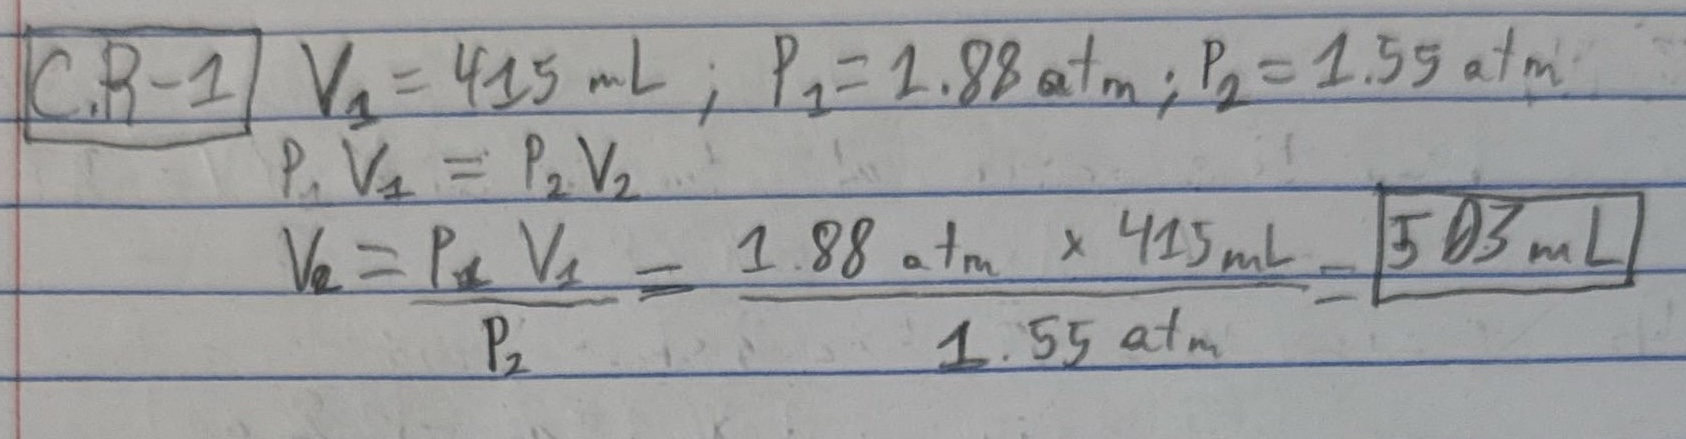
\includegraphics[width=\textwidth]{Answers Images/answer_C_R-1.jpg}
            \end{center}

    \pagebreak
    \section{Topic C Problem R-2}
        A balloon is filled with 3.85 L of oxygen at 31\unit{\celsius} and a pressure of 734 torr. 
        The balloon is then taken to the top of a mountain, where the pressure is 591 torr. 
        The volume of the oxygen is found to be 4.13 L. What is the temperature of the oxygen? 
        Give your answer in \unit{\celsius}.

        \subsection{Solution}
            \begin{center}
                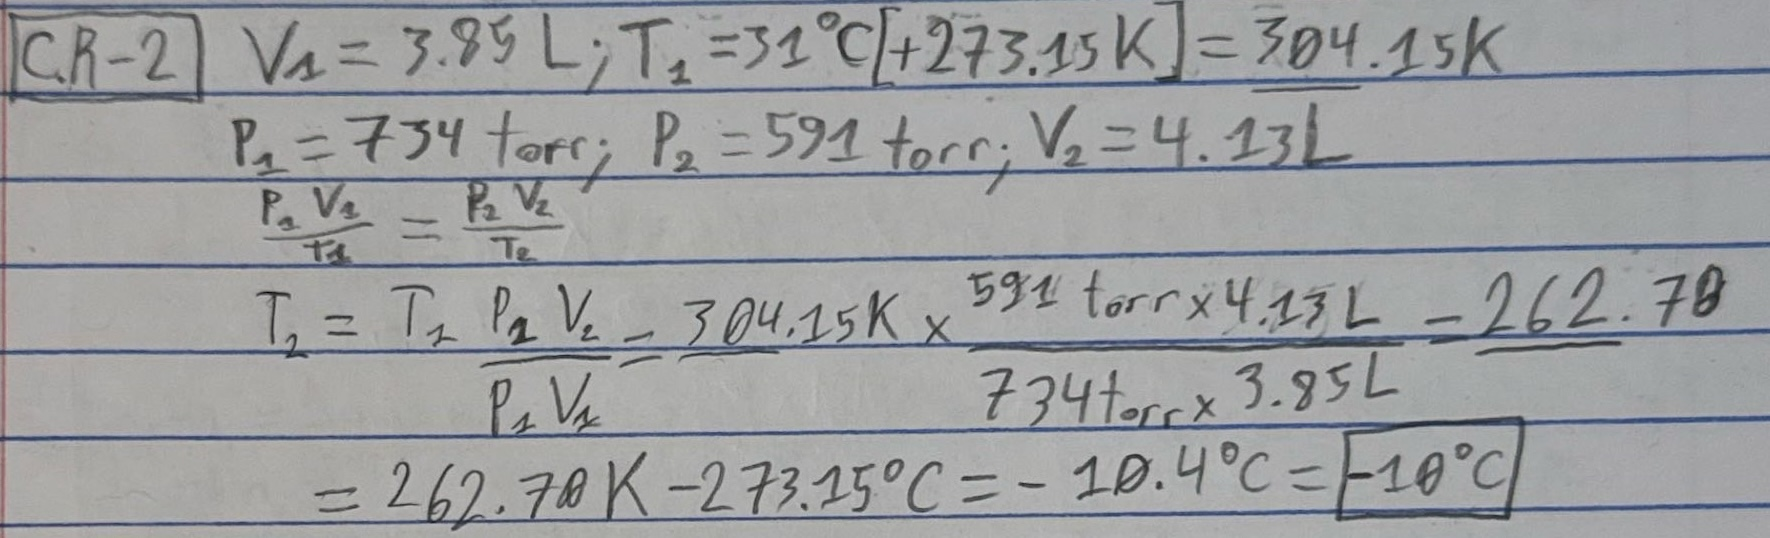
\includegraphics[width=\textwidth]{Answers Images/answer_C_R-2.jpg}
            \end{center}

    \pagebreak
    \section{Topic C Problem R-3}
        A container is filled with gaseous \ce{O2} at 21.4\unit{\celsius} (70.5$^\circ$F) and a pressure of 754 torr. 
        If the volume of the container is one gallon (3785 mL), what is the mass of the \ce{O2}?

        \subsection{Solution}
            \begin{center}
                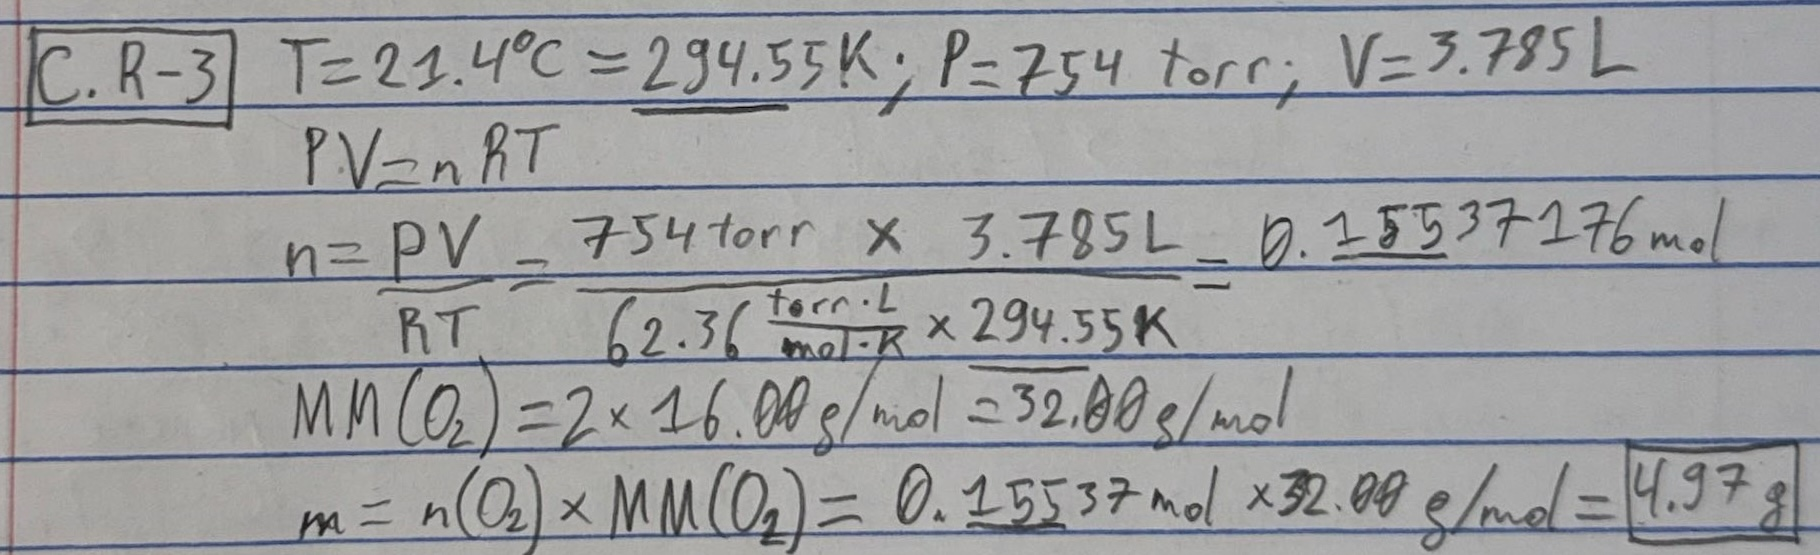
\includegraphics[width=\textwidth]{Answers Images/answer_C_R-3.jpg}
            \end{center}

    \pagebreak
    \section{Topic C Problem R-4}
        A container is filled with 25.3 g of gaseous \ce{CO2} at 31\unit{\celsius}. 
        If the carbon dioxide exerts a pressure of 3.88 atm, what is the volume of the container?

        \subsection{Solution}
            \begin{center}
                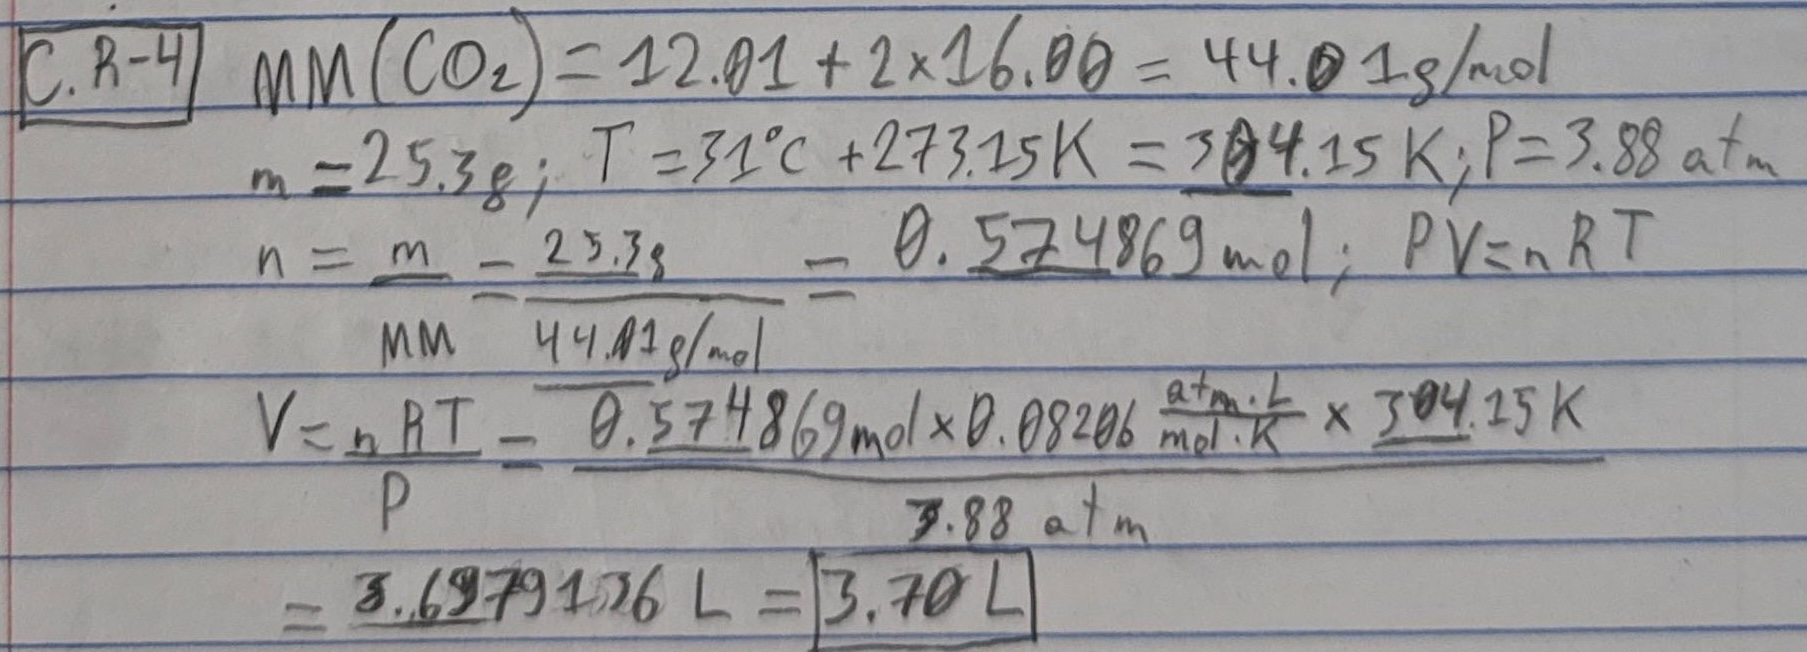
\includegraphics[width=\textwidth]{Answers Images/answer_C_R-4.jpg}
            \end{center}

    \pagebreak
    \section{Topic C Problem R-5}
        What is the density of gaseous carbon dioxide at 51\unit{\celsius} and a pressure of 855 torr?

        \subsection{Solution}
            \begin{center}
                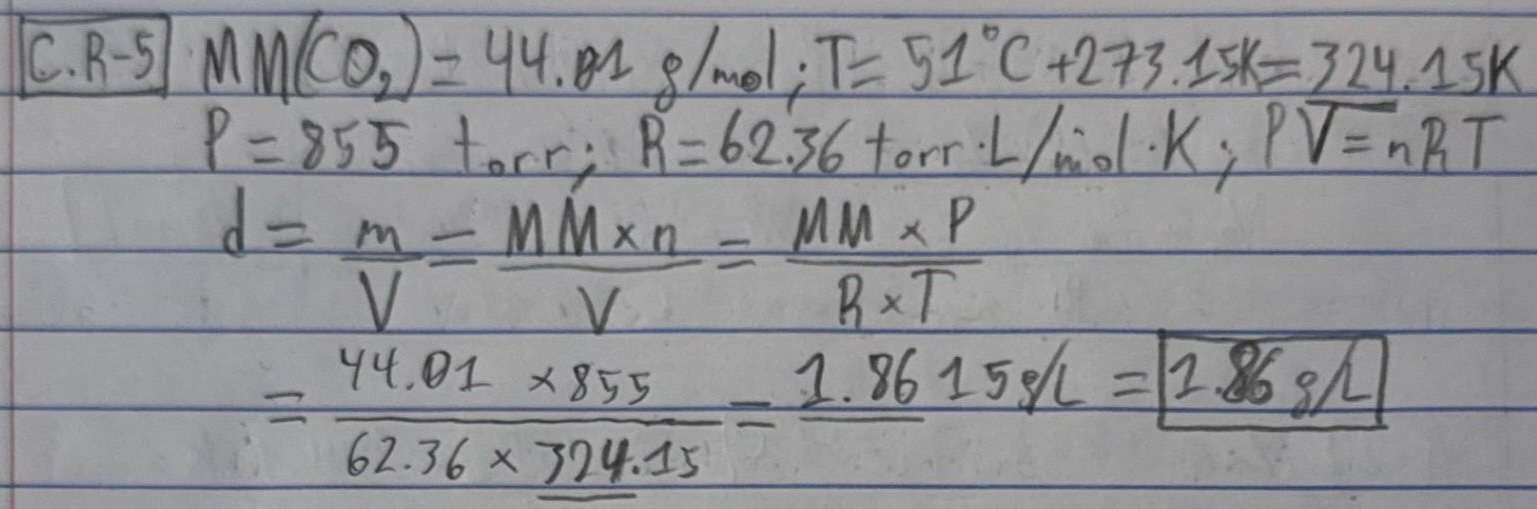
\includegraphics[width=\textwidth]{Answers Images/answer_C_R-5.jpg}
            \end{center}

    \pagebreak
    \section{Topic C Problem 1}
        A gaseous compound has the following composition: 85.63\% carbon, 14.37\% hydrogen. 
        The density of this compound is 1.63 g/L at 33.2\unit{\celsius} and a pressure of 739 torr. 
        What is the molecular formula of the compound?

        \subsection{Solution}
            \begin{center}
                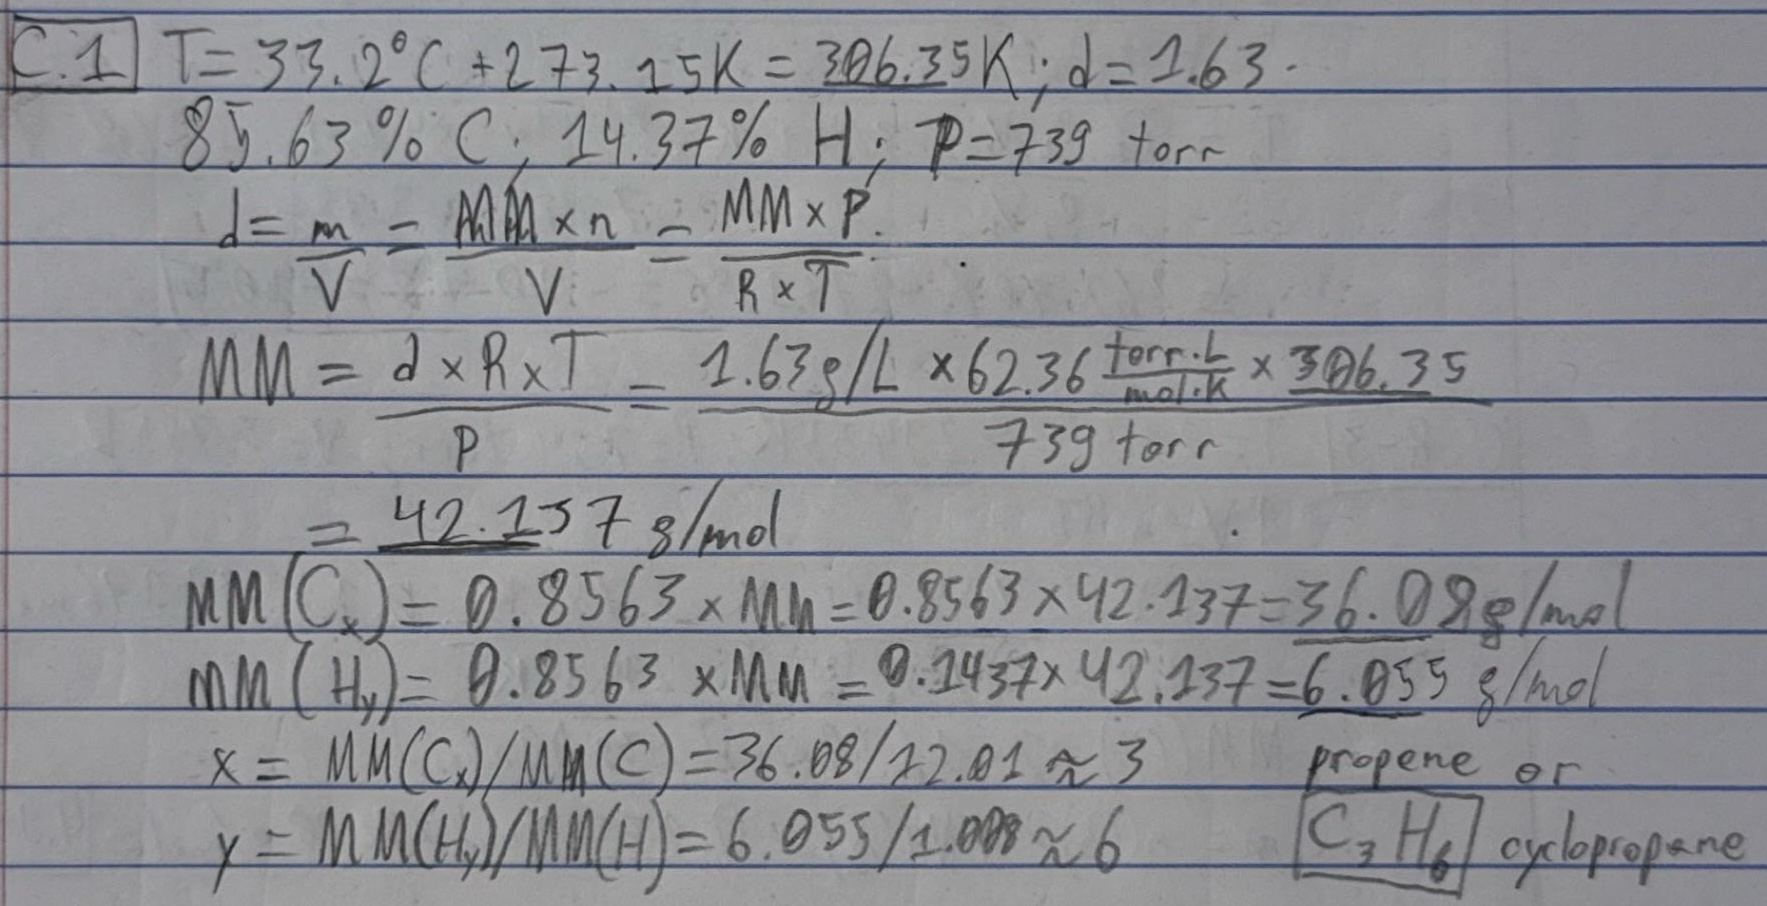
\includegraphics[width=\textwidth]{Answers Images/answer_C_1.jpg}
            \end{center}

    \pagebreak
    \section{Topic C Problem 2}
        Copper reacts with nitric acid as shown below:
        \begin{gather}
            \ce{Cu(s) + 4 HNO3(aq) -> Cu(NO3)2(aq) + 2 NO2(g) + 2 H2O(l)}
        \end{gather}
        If 4.71 g of copper reacts with excess 3 M nitric acid, what volume of nitrogen dioxide will be formed at 31\unit{\celsius} and 1.022 atm?

        \subsection{Solution}
            \begin{center}
                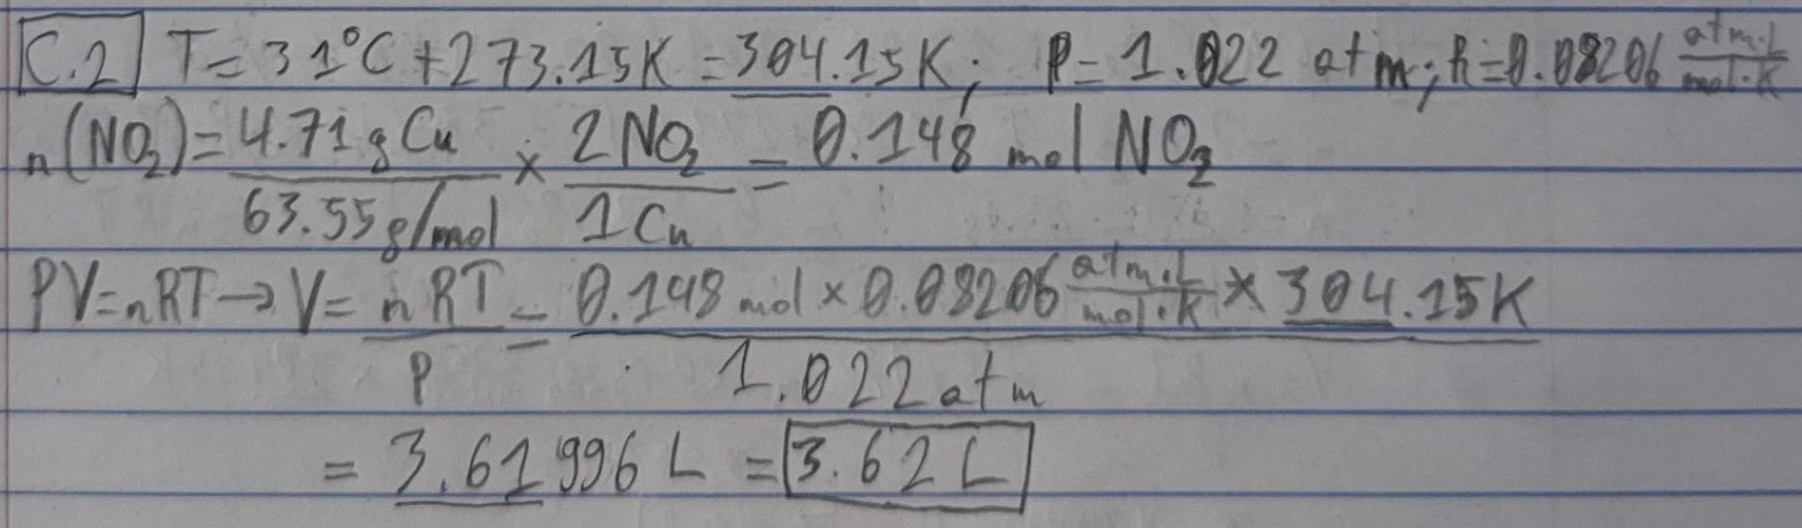
\includegraphics[width=\textwidth]{Answers Images/answer_C_2.jpg}
            \end{center}

    \pagebreak
    \section{Topic C Problem 3}
        Consider the following reaction:
        \begin{gather}
            \ce{4 Cr2+(aq) + O2(g) + 4 H+(aq) -> 4 Cr3+(aq) + 2 H2O(l)}
        \end{gather}
        A container that holds 562 mL of gaseous oxygen at 21\unit{\celsius} is prepared. 
        Then, 21.3 mL of a solution that contains 0.131 M \ce{Cr^2+} ions is added to the container. 
        After the reaction, the pressure of the oxygen in the container is found to be 119 torr and the temperature is still 21\unit{\celsius}.
        What was the pressure of oxygen in the container before the \ce{Cr^2+} solution was added? 
        (You can assume that \ce{H+} is present in excess.)

        \subsection{Solution}
            \begin{center}
                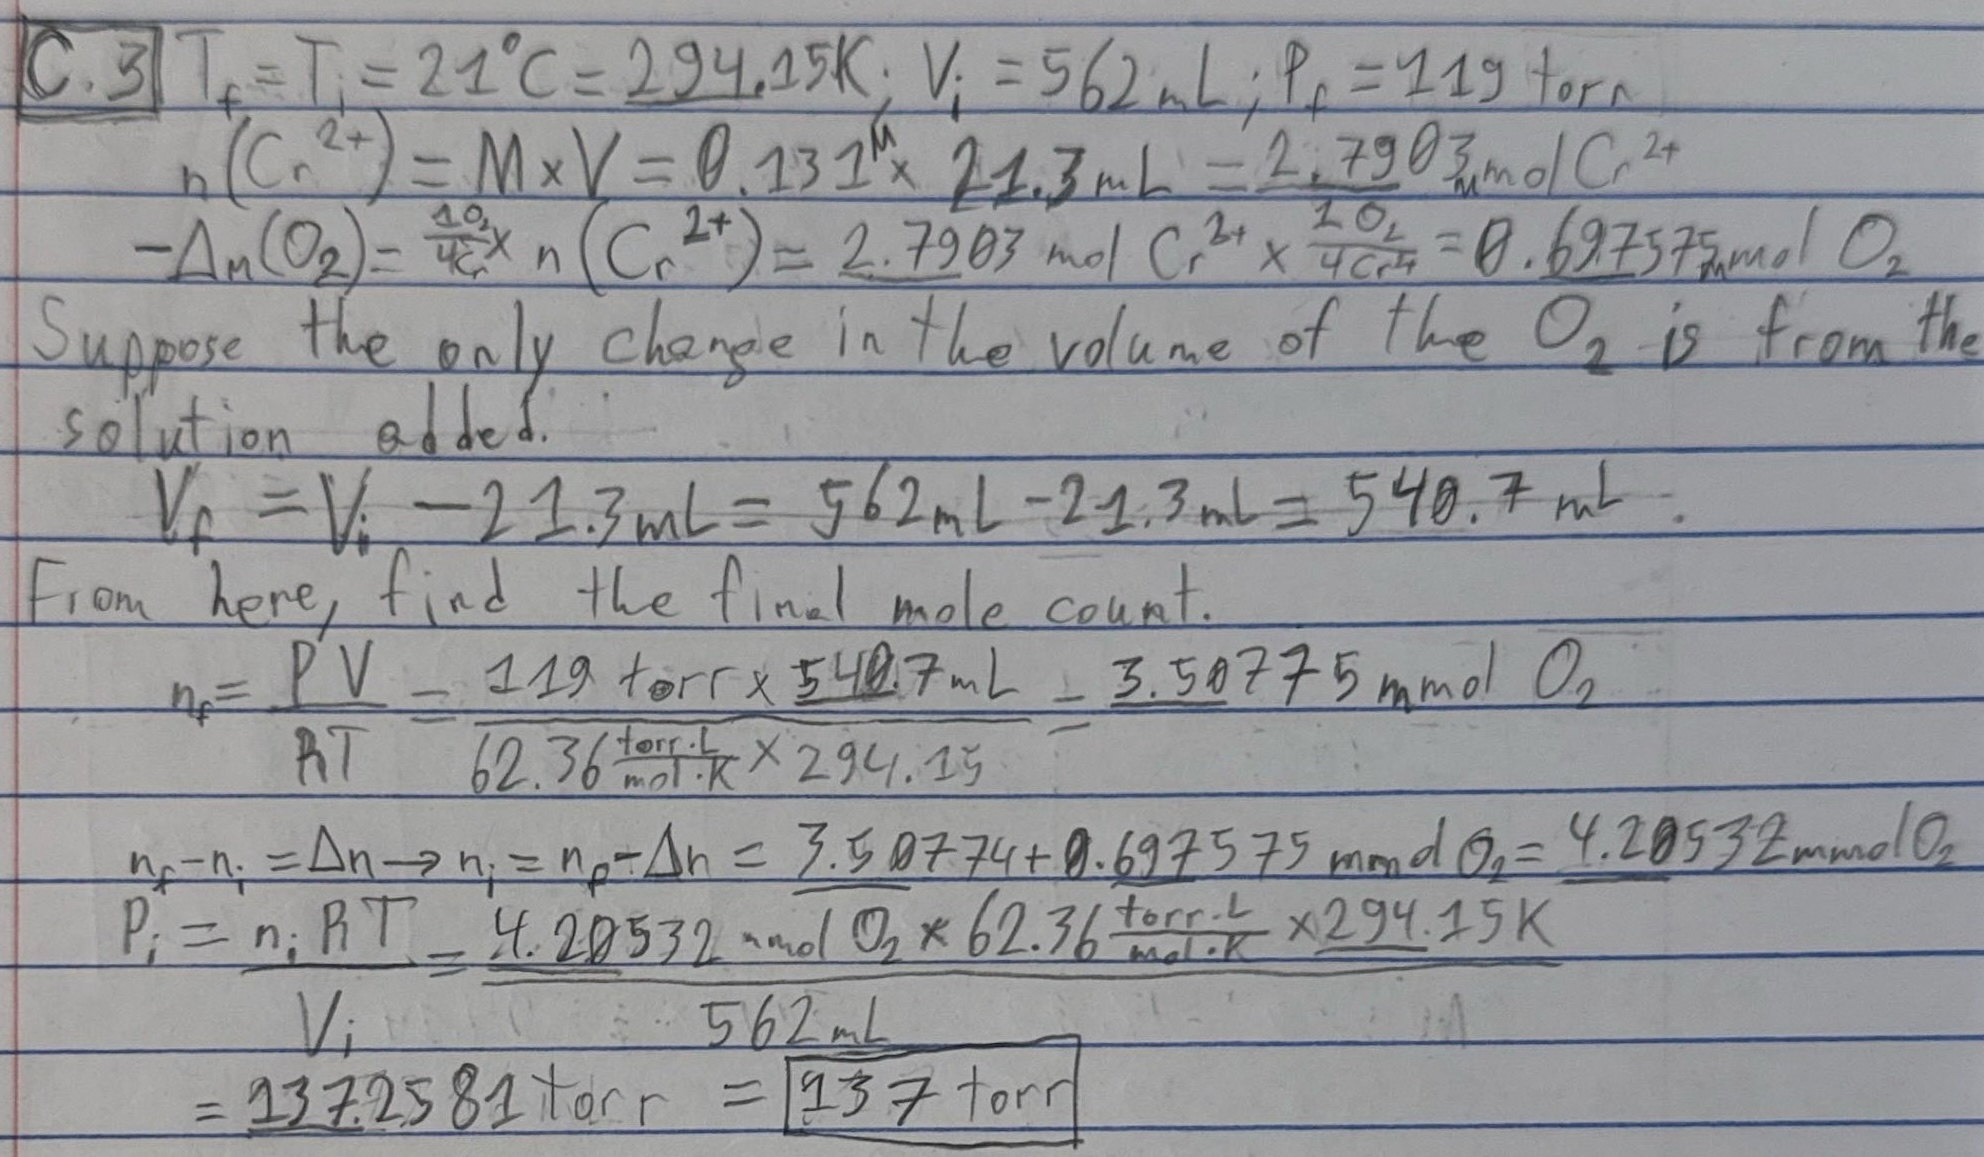
\includegraphics[width=\textwidth]{Answers Images/answer_C_3.jpg}
            \end{center}

    \pagebreak
    \section{Topic C Problem 4}
        A chemist puts 200.0 mL of water into a 2.50 L container, and adds enough gaseous \ce{H2S} to give a pressure of 180.2 torr at a temperature of 13.0\unit{\celsius}. 
        Some of the \ce{H2S} then dissolves in the water, causing the pressure in the container to drop to 155.9 torr. 
        The temperature remains constant throughout this experiment. 
        What is the molar concentration of \ce{H2S} in the water at the end of the experiment?

        \subsection{Solution}
            \begin{center}
                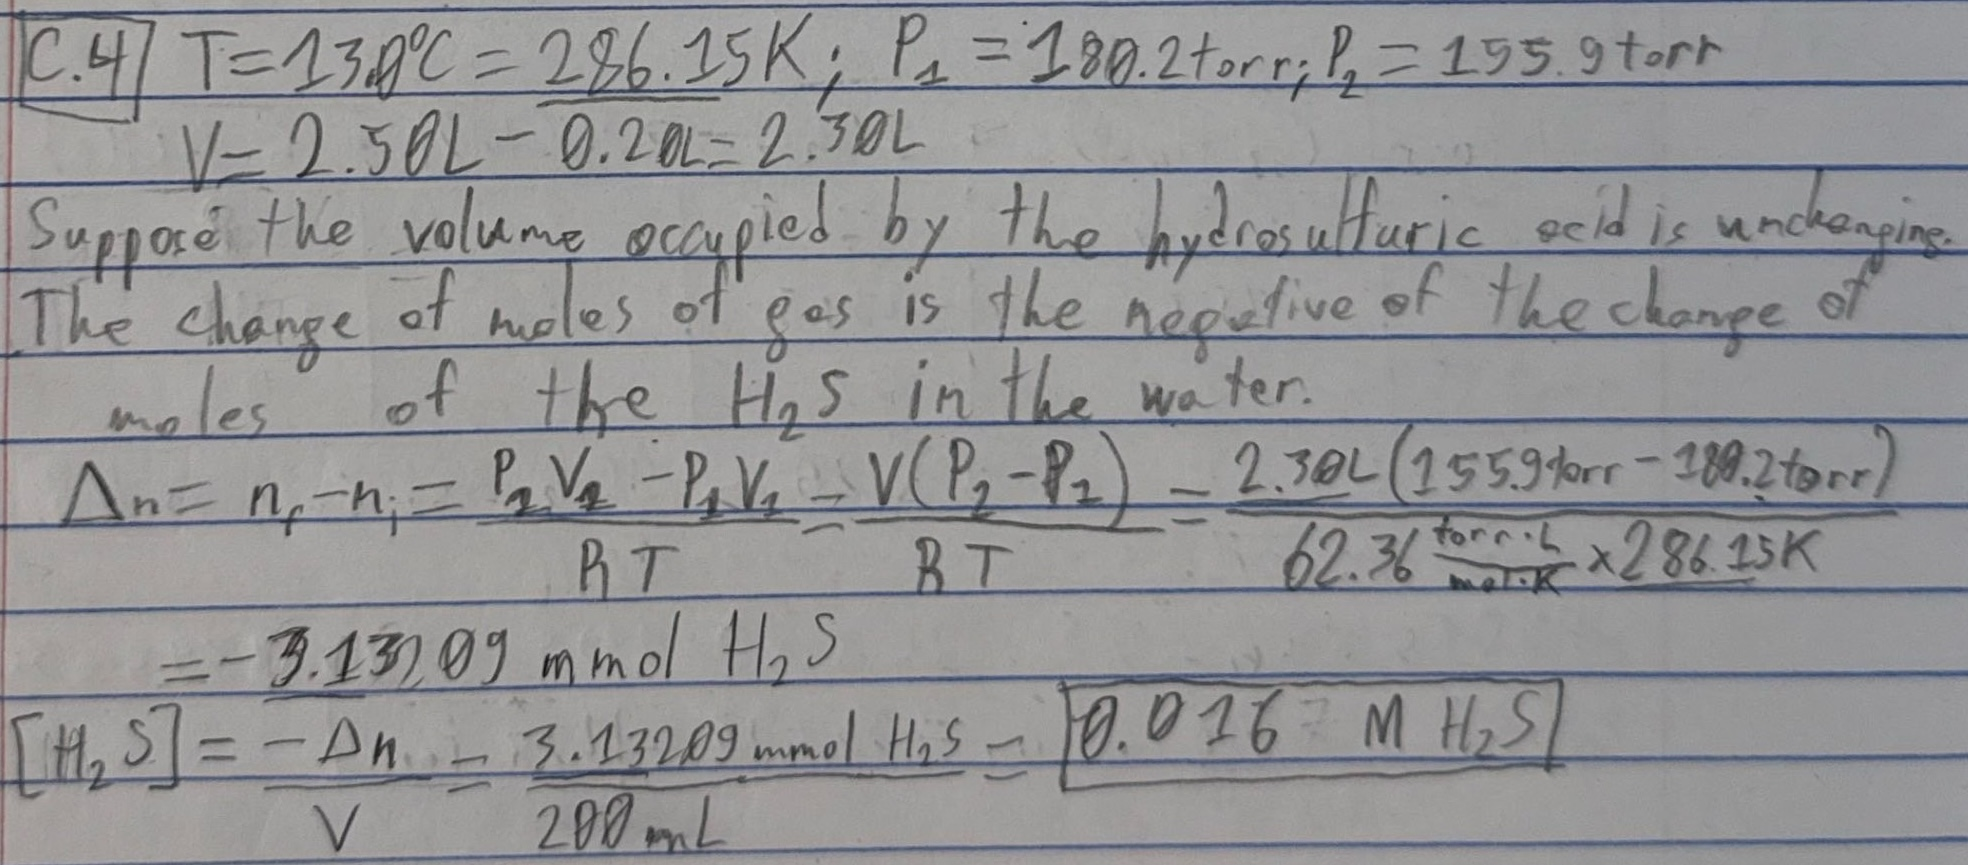
\includegraphics[width=\textwidth]{Answers Images/answer_C_4.jpg}
            \end{center}

    \pagebreak
    \section{Topic C Problem 5}
        Consider the apparatus pictured below, which consists of two containers separated by a valve.
        \begin{center}
            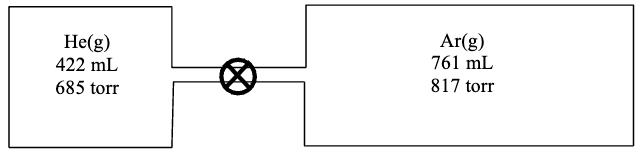
\includegraphics{picture_C-5.png}
        \end{center}
        Assuming that the two gases are the same temperature and that the temperature does not change, what will be the total final pressure in the system after the valve is opened and the gases mix completely?

        \subsection{Solution}
            \begin{center}
                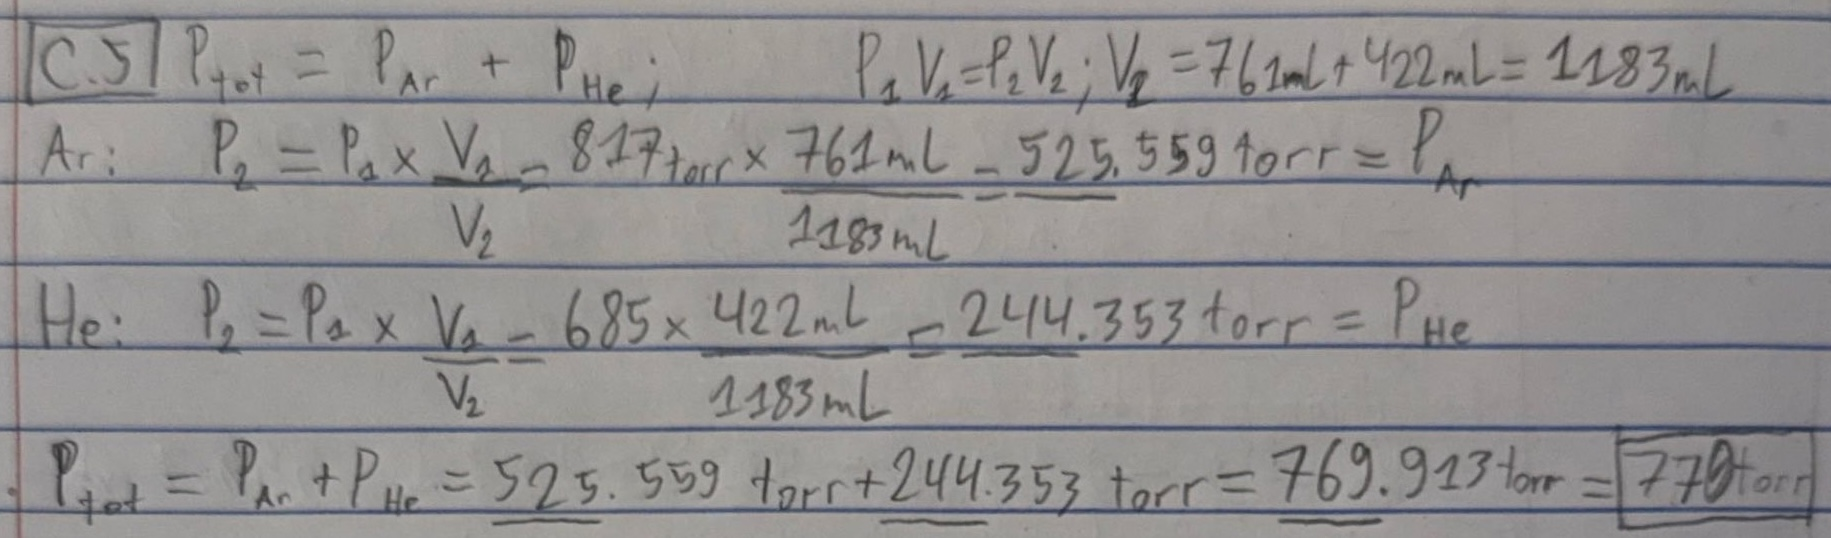
\includegraphics[width=\textwidth]{Answers Images/answer_C_5.jpg}
            \end{center}

    \pagebreak
    \section{Topic C Problem 6}
        Complete the following ICE table. 
        All of the reactants and products for this reaction are gases, and the temperature and volume are constant during the reaction.

        \begin{center}
            \begin{tabular}{|l|c@{}c@{}c@{}c@{}c@{}c@{}c|}
                \hline
                torr &   \ce{C2H6} & ${}+{}$ & \ce{7 F2} & ${}\rightarrow{}$ & \ce{2 CF4} & ${}+{}$ & \ce{6 HF}\\
                \hline
                Initial pressure (torr) &   127.3       &&          329.5                       &&  89.1        &&          0       \\
                Change (torr)           &               &&                                      &&              &&                  \\
                Ending pressure (torr)  &               &&                                      &&              &&                  \\
                \hline
            \end{tabular}
        \end{center}

        \subsection{Solution}
            \begin{center}
                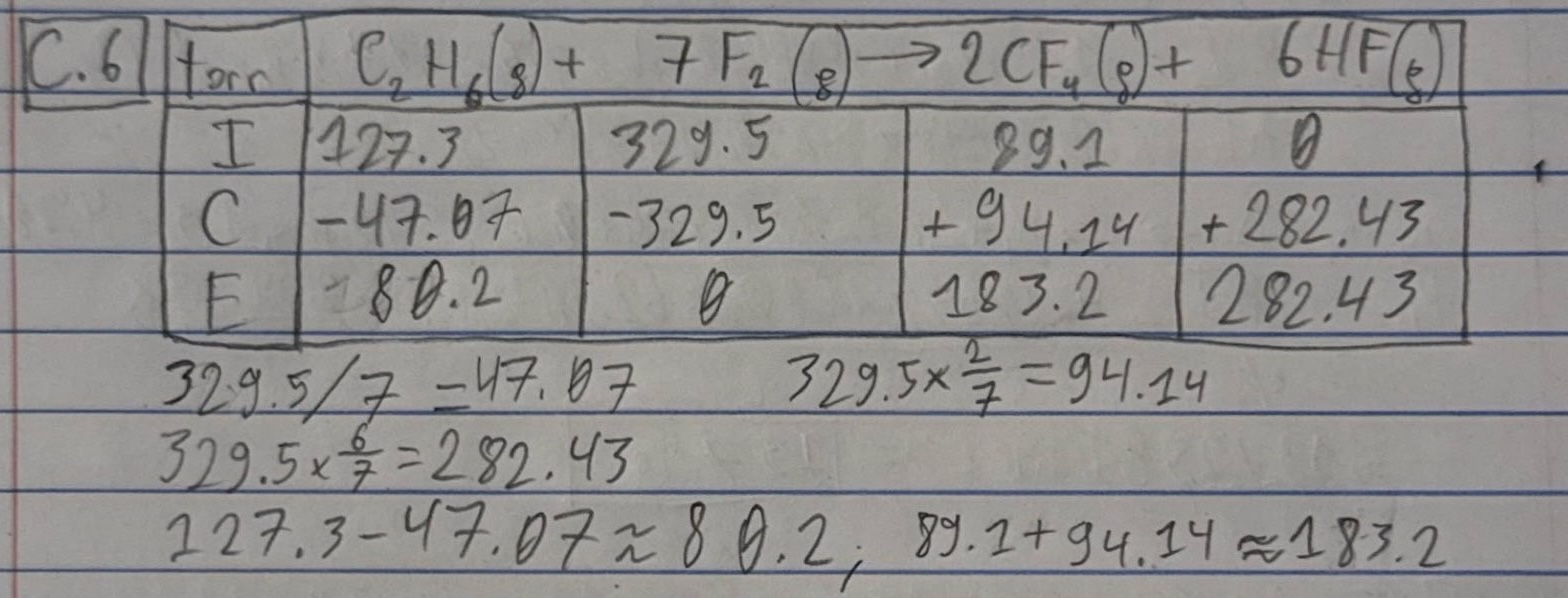
\includegraphics[width=\textwidth]{Answers Images/answer_C_6.jpg}
            \end{center}

    \pagebreak
    \section{Topic C Problem 7}
        At 30\unit{\celsius}, propylene (C3H6) reacts with chlorine as follows:
        \begin{equation}
            \ce{C3H6(g) + 9 Cl2(g) -> 3 CCl4(l) + 6 HCl(g)}
        \end{equation}
        A mixture containing 15.5 torr of C3H6 and 174.5 torr of Cl2 is allowed to react at 30\unit{\celsius}. 
        What will be the total gas pressure in the container when the reaction is complete? 
        You may assume that the volume and temperature are constant.

        \subsection{Solution}
            \begin{center}
                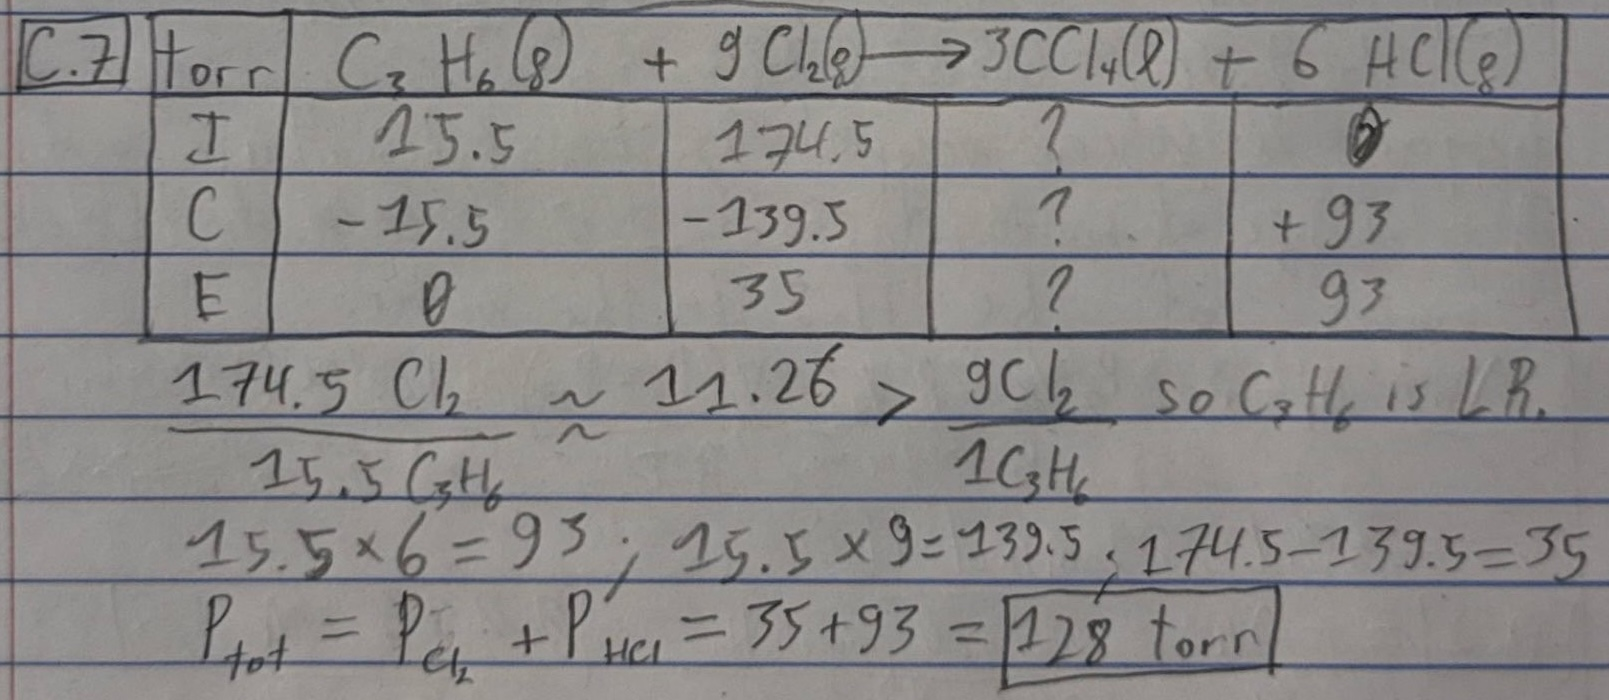
\includegraphics[width=\textwidth]{Answers Images/answer_C_7.jpg}
            \end{center}

    \pagebreak
    \section{Topic C Problem 8}
        Consider the apparatus pictured below, which consists of two containers separated by a valve.
        \begin{center}
            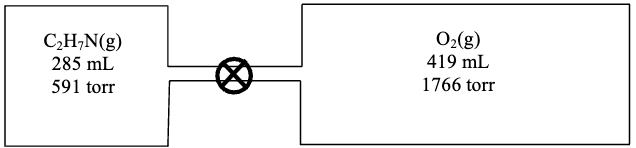
\includegraphics{picture_C-8.png}
        \end{center}
        The valve is opened and the gases react as follows (note that the temperature is high enough that
        the water is produced as a gas):
        \begin{equation}
            \ce{4 C2H7N(g) + 15 O2(g) -> 8 CO2(g) + 14 H2O(g) + 2 N2(g)}
        \end{equation}
        What will be the total pressure in the apparatus when the reaction has gone to completion?
        Assume that the temperature does not change.

        \subsection{Solution}
            \begin{center}
                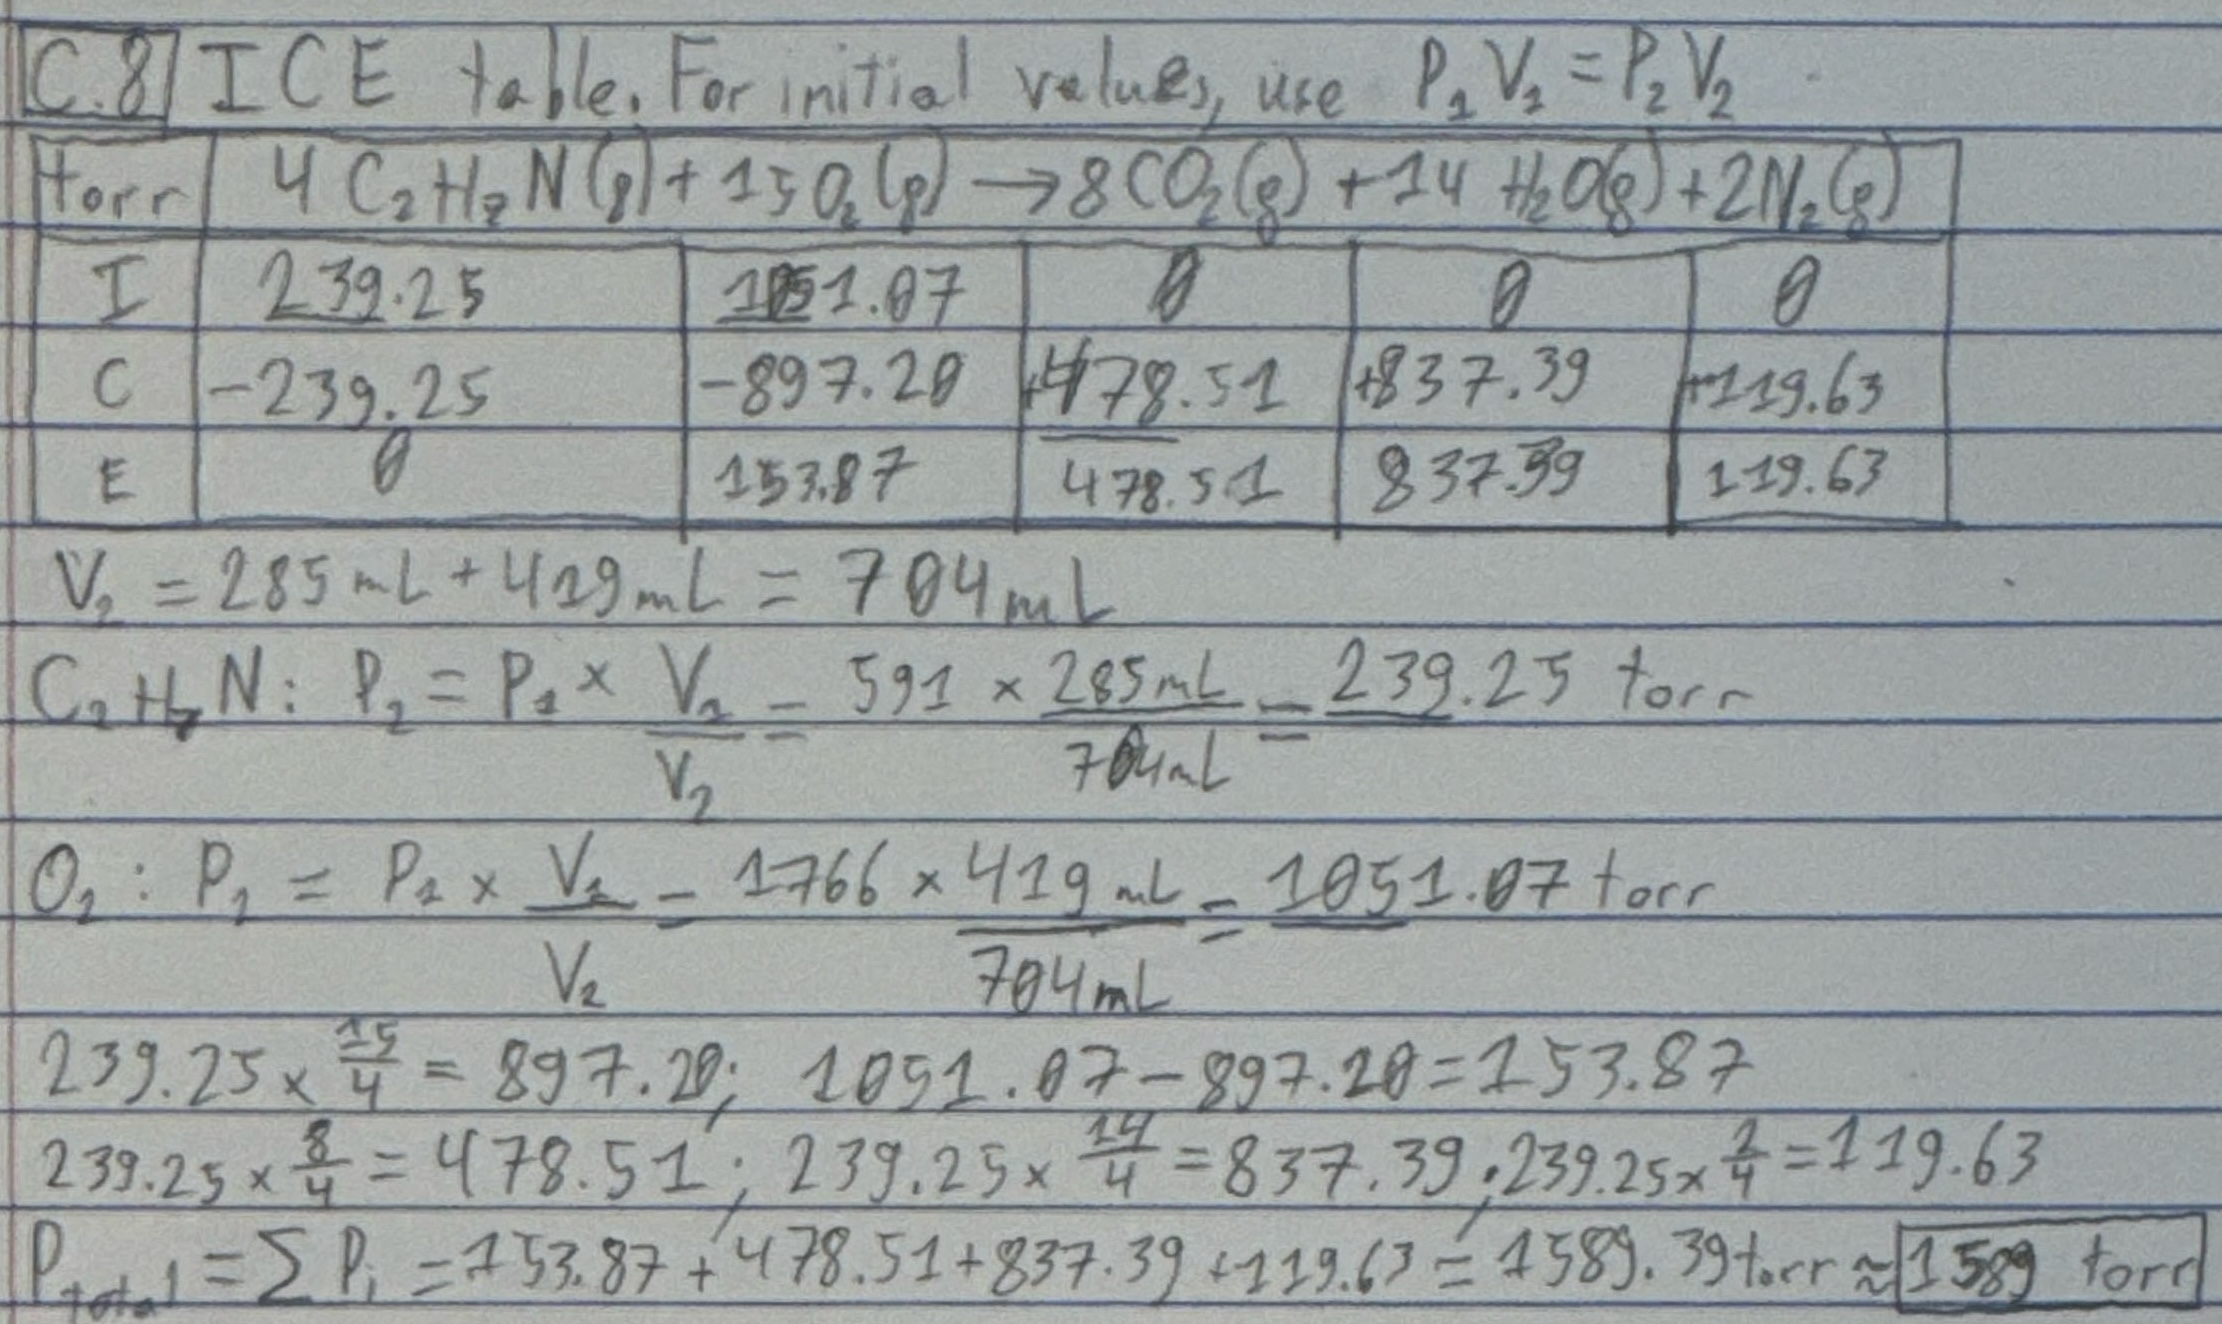
\includegraphics[width=\textwidth]{Answers Images/answer_C_8.jpg}
            \end{center}

    \pagebreak
    \section{Topic C Problem 9}
        Consider the apparatus pictured below, which consists of two containers separated by a valve.
        \begin{center}
            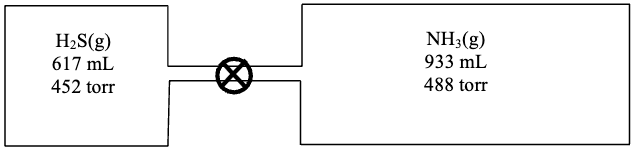
\includegraphics{picture_C-9.png}
        \end{center}
        The valve is opened and the gases react as follows:
        \begin{equation}
            \ce{H2S(g) + 2 NH3(g) -> (NH4)2S(s)}
        \end{equation}
        What will be the total pressure in the apparatus when the reaction has gone to completion?
        Assume that the temperature does not change.

        \subsection{Solution}
            \begin{center}
                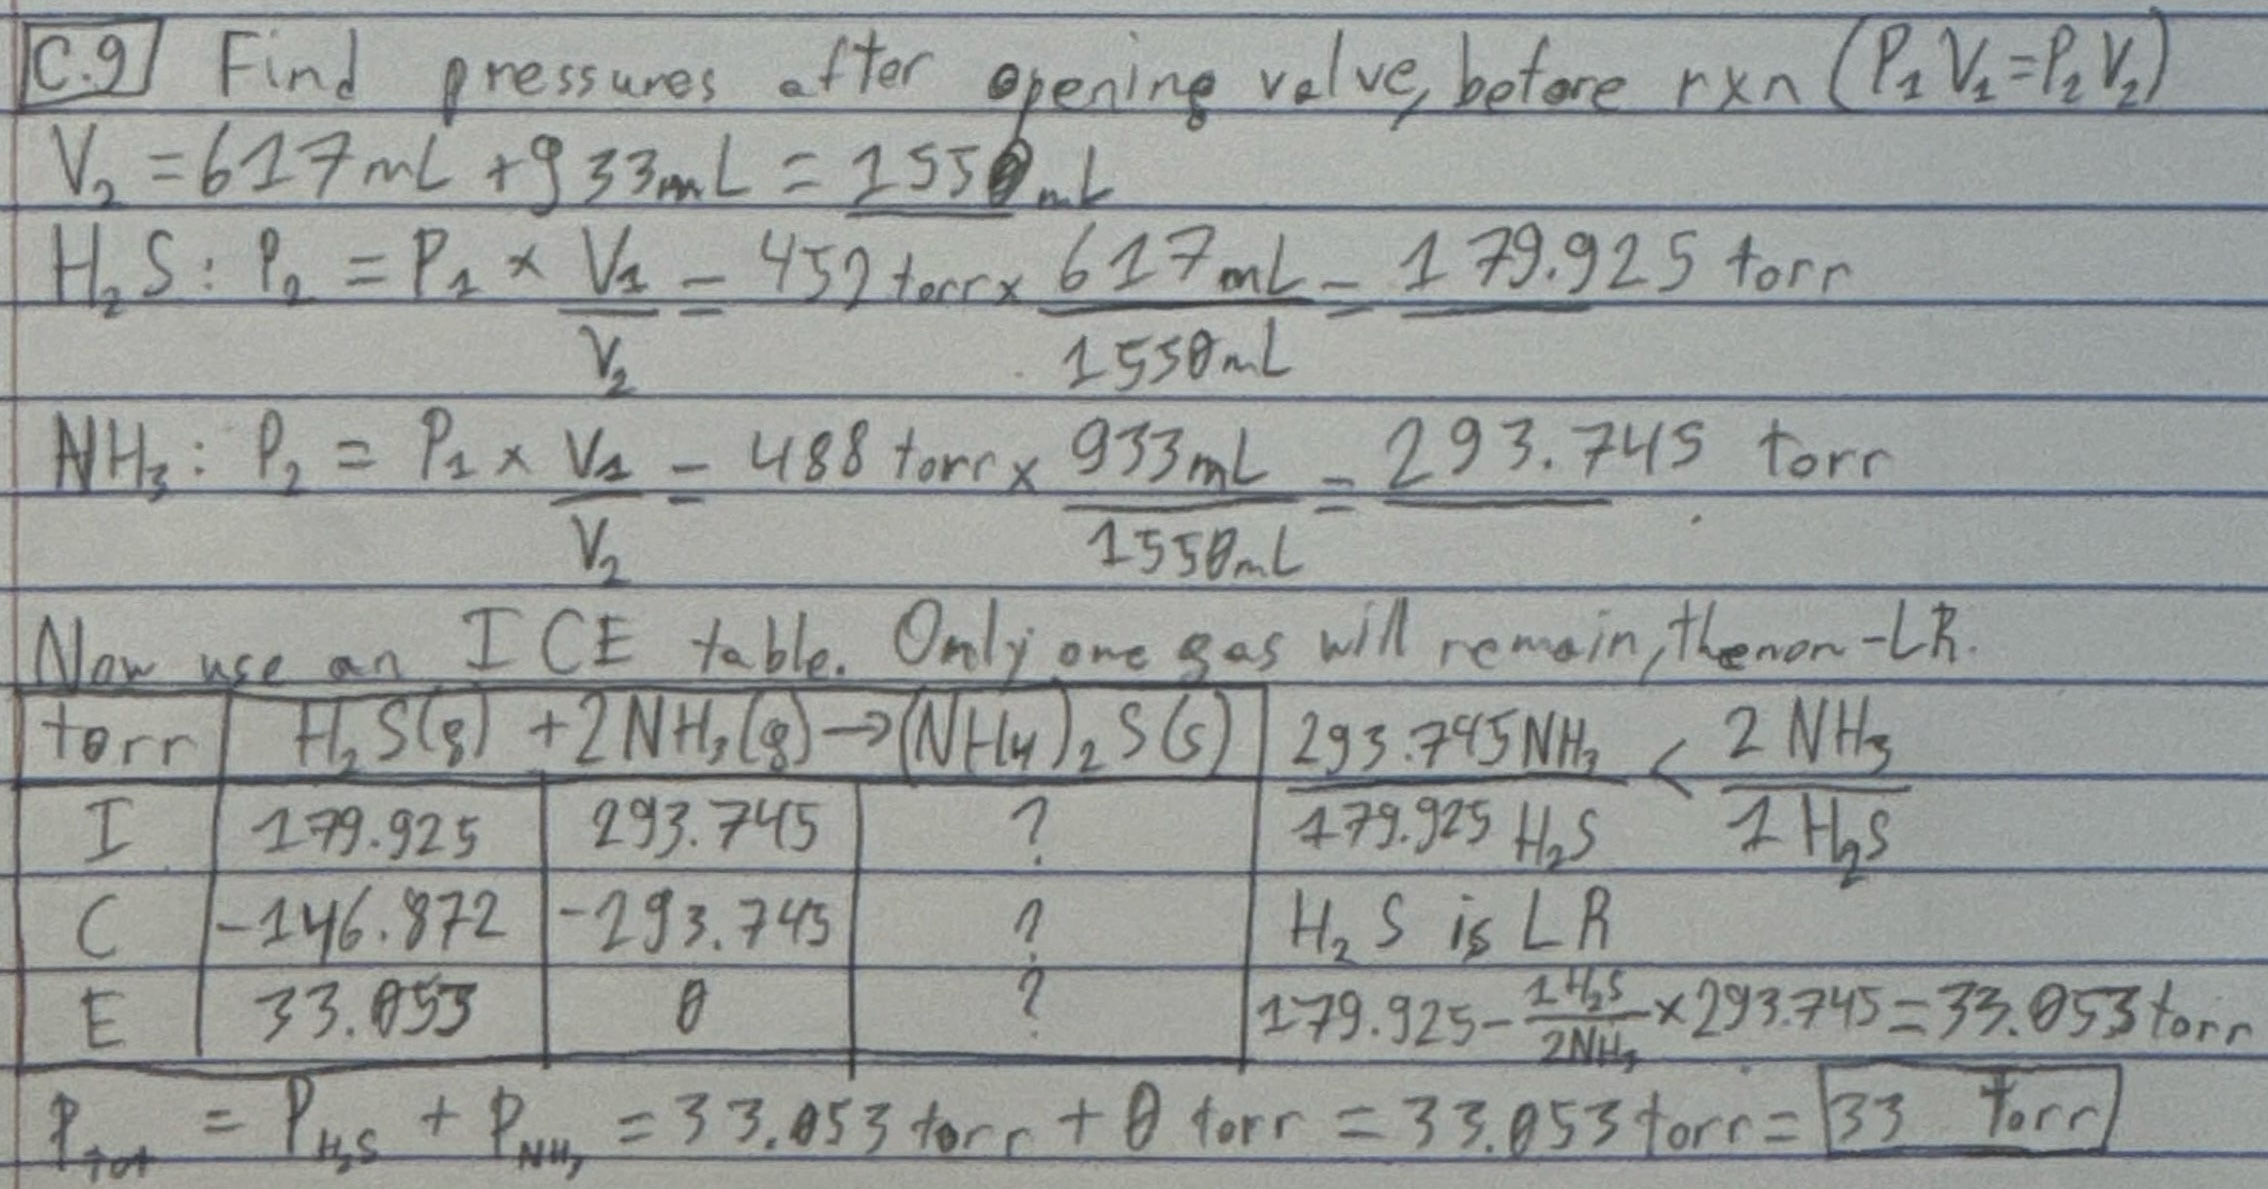
\includegraphics[width=\textwidth]{Answers Images/answer_C_9.jpg}
            \end{center}

    \pagebreak

    \tableofcontents
\end{document}